\documentclass{article}
\usepackage[utf8]{inputenc}
\usepackage{amssymb}
\usepackage{comment}
\usepackage{graphicx}
\usepackage{amsmath,amsfonts,amssymb,amsthm}
\usepackage{mathtools}
\usepackage{commath}
\usepackage{listings}


\title{Homework 3}
\author{Vladimir Frants, Yunhua Zhao, Mohamed Ben Zid}
\date{October 2020}

\begin{document}

\maketitle

\section{Exercise 3.2}

\subsection{a)} 

We want to represent the specified recursion in the form:

$$\theta_{n+1} = \theta_{n} + \epsilon_{n}Y_{n}$$, 

where $\{Y_{n}\}$ is a stochastic process depending on the random variable $\xi_{n}\in\{A_{lose}, B_{lose}, A_{win}, B_{win}\}$. Values of the $\xi_n$ represent one of the four possibilities for each step $n$.

In situations when $\xi_n\in\{A_{lose}, B_{lose}\}$ we do not update estimate of the $\theta$, for $\xi_n=A_{win}$ we add $\epsilon_{n}\cdot(1-\theta_{n})$ to our estimate, and for $\xi_{n}=B_{win}$ we subtract $\epsilon_n\theta_{n}$. This could be achieved with:

$$Y_{n}(\xi_{n})=\mathrm{1}_{(\xi_{n}=A_{win})}\cdot(1-\theta_{n}) - \mathrm{1}_{(\xi_{n}=B_{win})}\cdot\theta_{n}$$


Given initial value $\theta_0$, recursively define the feedback process ${Y_n}$ through $$ \theta_{n+1} = \theta_n+\epsilon_nY_n $$
with either fixed step size $\epsilon$ or decreasing step size, where we typically assume that 
$$ \sum_{n=1}^{\infty}\epsilon_n = +\infty $$
$$ \sum_{n=1}^{\infty}\epsilon_n^2 < \infty $$
and $Y_n$ given via the feedback function
$$ Y_n = \phi(\xi(\theta_n),\theta_n) $$
 
We assume that all random variables, that is, $\theta0$ and $ ({\xi_n(\theta):n>=0, \theta\in\Theta}) $, are defined on a probability
space. Running the stochastic approximation algorithm, we observe the underlying
sequence
$$ \xi_0(\theta_0), \xi_1(\theta_1),... $$ 
Here in the problem, 
$$ \xi_1(\theta_1) = (0_{initial lose},(1-\theta_{0})_{initial A wins}, (-\theta_{0})_{initial B wins}) $$
$$ \xi_2(\theta_2) = (0_{1th lose},(1-\theta_{1})_{1th A wins}, (-\theta_{1})_{1th B wins}) $$
$$ \xi_3(\theta_3) = (0_{2th lose},(1-\theta_{2})_{2th A wins}, (-\theta_{2})_{2th B wins}) $$
$$ \xi_2(\theta_4) = (0_{3th lose},(1-\theta_{3})_{3th A wins}, (-\theta_{3})_{3th B wins}) $$
and so on, ...  \\

\subsection{b)} 

So we have the stochastic approximation of the form:

$$\theta_{n+1}=\theta_{n} + \epsilon_{n}\cdot (\mathrm{1}_{(\xi_{n}=A_{win})}\cdot(1-\theta_{n}) - \mathrm{1}_{(\xi_{n}=B_{win})}\cdot\theta_{n})$$

Assuming that there is no bias term the target field function we have target vector field (scalar in our case):

$$G(\theta_{n})=\mathrm{1}_{(\xi_{n}=A_{win})}\cdot(1-\theta_{n}) - \mathrm{1}_{(\xi_{n}=B_{win})}\cdot\theta_{n}$$

because $$ \theta_{n+1} = \theta_n+\epsilon_nY_n $$ 
set $Y_n(\xi_n(\theta_n))$ is the independent sequences of unbiased estimators of the target vector field, where
$$Y_n(\xi_n(\theta_n)) = (0_{n-1-th lose}, (1-\theta_{n-1})_{n-1-th A wins}, (-\theta_{n-1})_{n-1-th B wins}) $$


\subsection{c)} 

\textbf{Under} strict monotonicity, if choose A win, $Y_n=\xi_n(\theta_n) = 1-\theta_n$ the chosen direction the gradient is bigger than 0, which is always the grow direction;  \\
\textbf{And} the probability that B win,  $Y_n=\xi_n(\theta_n) = -\theta_n$ is always a descent direction, which is always the decent direction. \\
\textbf{So} this means that the field is coercive for the well-posed optimization problem.  \\

\subsection{d)}

For the case of constant $\epsilon$:

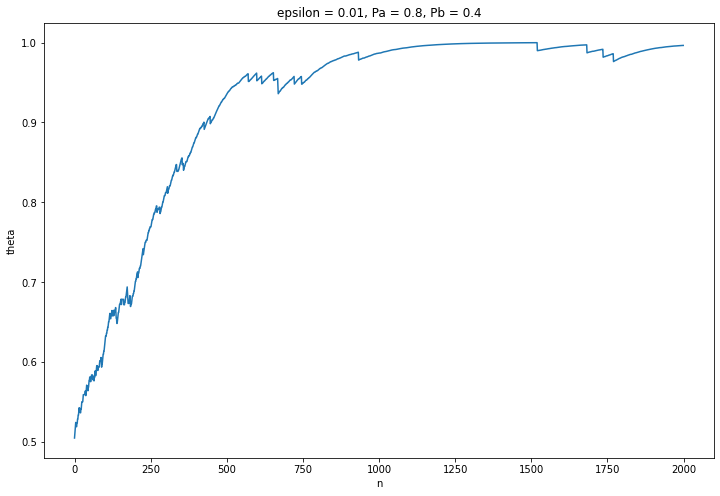
\includegraphics[width=0.9\linewidth]{const_a.png}\\

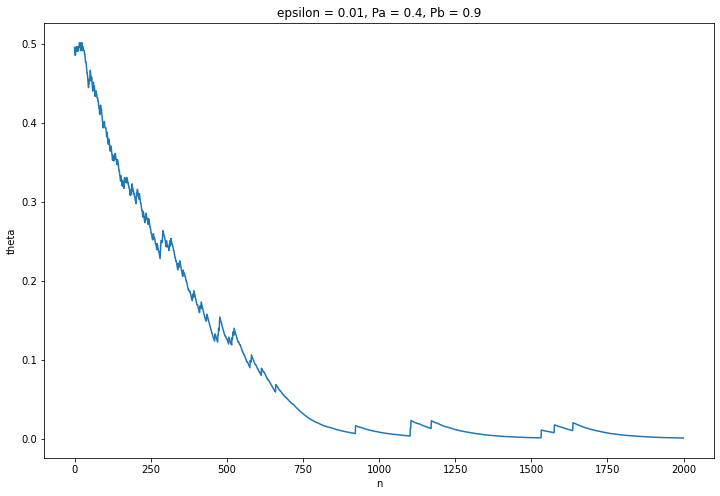
\includegraphics[width=0.9\linewidth]{const_b.png}\\

For the case of $\epsilon=\frac{1}{n}$:

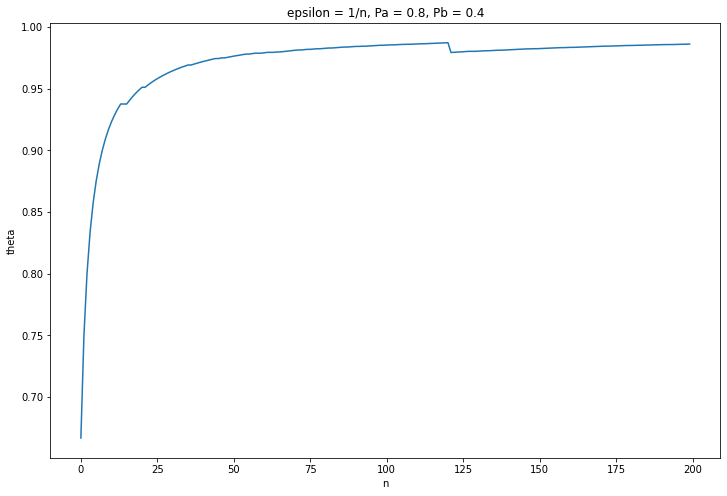
\includegraphics[width=0.9\linewidth]{repr_a.png}\\
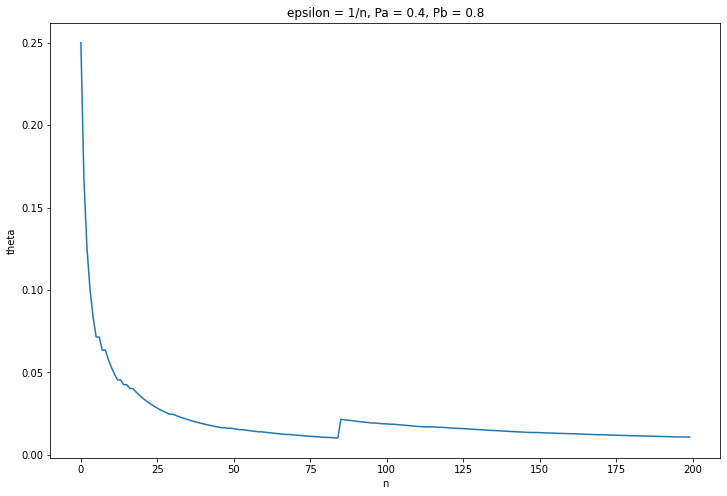
\includegraphics[width=0.9\linewidth]{repr_b.png}\\

It could be seen that procedure for $\epsilon=\frac{1}/{n}$ converges faster.

We use this python script to generate the plots:

\begin{lstlisting}[language=python, caption={Resolve contention}, label={main_1}, basicstyle=\small]

import os
import random
import matplotlib.pyplot as plt

random.seed(18)

def bandit(pA, pB, thetan):
  if random.random() < thetan:
    # arm A
    if random.random() < pA:
      return 'Awin'
    else:
      return 'Alose'
  else:
    if random.random() < pB:
      return 'Bwin'
    else:
      return 'Blose'
      
probA = 0.8
probB = 0.4

theta = 0.5
eps = 0.01
thetas = []
ns = []
for n in range(2000):
  event = bandit(probA, probB, thetan=theta)
  if event == 'Awin':
    theta += eps*(1 - theta)
  if event == 'Bwin':
    theta -= eps*theta

  ns.append(n)
  thetas.append(theta)

plt.figure(figsize=(12, 8))
plt.title('epsilon = {}, Pa = {}, Pb = {}'.format(eps, probA, probB))
plt.plot(ns, thetas)
plt.xlabel('n')
plt.ylabel('theta')

probA = 0.4
probB = 0.9

theta = 0.5
eps = 0.01
thetas = []
ns = []
for n in range(2000):
  event = bandit(probA, probB, thetan=theta)
  if event == 'Awin':
    theta += eps*(1 - theta)
  if event == 'Bwin':
    theta -= eps*theta

  ns.append(n)
  thetas.append(theta)

plt.figure(figsize=(12, 8))
plt.title('epsilon = {}, Pa = {}, Pb = {}'.format(eps, probA, probB))
plt.plot(ns, thetas)
plt.xlabel('n')
plt.ylabel('theta')


probA = 0.8
probB = 0.4

theta = 0.5
thetas = []
ns = []
for n in range(200):
  event = bandit(probA, probB, thetan=theta)
  if event == 'Awin':
    theta += (1/(n+3))*(1 - theta)
  if event == 'Bwin':
    theta -= (1/(n+3))*theta

  ns.append(n)
  thetas.append(theta)

plt.figure(figsize=(12, 8))
plt.title('epsilon = 1/n, Pa = {}, Pb = {}'.format(probA, probB))
plt.plot(ns, thetas)
plt.xlabel('n')
plt.ylabel('theta')

probA = 0.4
probB = 0.8

theta = 0.5
thetas = []
ns = []
for n in range(200):
  event = bandit(probA, probB, thetan=theta)
  if event == 'Awin':
    theta += (1/(n+2))*(1 - theta)
  if event == 'Bwin':
    theta -= (1/(n+2))*theta

  ns.append(n)
  thetas.append(theta)

plt.figure(figsize=(12, 8))
plt.title('epsilon = 1/n, Pa = {}, Pb = {}'.format(probA, probB))
plt.plot(ns, thetas)
plt.xlabel('n')
plt.ylabel('theta')

\end{lstlisting}

\section{Exercise 4.4}

Show that  for a random variable x with finite variance
$$ \nabla J(\theta) = (-E[Z(X)-\theta_1-\theta_2X], -E[XZ(X)-\theta_1X-\theta_2X^2])^\intercal  \ \ (1) $$
$$J(\theta) = \frac{1}{2}E[(Z(X)-(\theta_1+\theta_2X))^2] \ \ (2)$$
Which we could get:
$$\frac{\partial J(\theta)}{\partial \theta_1} = -E[Z(X)-(\theta_1-\theta_2X)] \ \ (3) $$
$$\frac{\partial J(\theta)}{\partial \theta_2} = -E[XZ(X)-\theta_1X-\theta_2X^2]  \ \ (4)$$
For each $x_n$ we obtain a corresponding random observation $ \xi_n=Z(x_n)$ \\
$$ E(Z(x_n)) = h(x_n) $$
The feedback function is 
 $$ Y_n = (\xi_n-\theta_n(1)-\theta_n(2)x_n)(1,x_n)^\intercal \ \ (5)$$
 
Because $x_n$ and $Z(x_n)$ are random, so $Y_n$ is independent:
\begin{flushleft}
$ E[Y_n|\mathfrak{F_{n-1}}] = E[(\xi_n-\theta_n(1)-\theta_n(2)x_n)(1,x_n)^\intercal] $  \\
$ \ \ \ \ \ \ \ \ \ \ \ \ \ \ \ \ =E[(Z(x_n)-\theta_n(1)-\theta_n(2)x_n, x_nZ(x_n)-\theta_n(1)x_n-\theta_n(2)x_n^2)^\intercal] $  \\
$ \ \ \ \ \ \ \ \ \ \ \ \ \ \ \ \ =(E[Z(x_n)-\theta_n(1)-\theta_n(2)x_n], E[x_nZ(x_n)-\theta_n(1)x_n-\theta_n(2)x_n^2])^\intercal $  \\
$ \ \ \ \ \ \ \ \ \ \ \ \ \ \ \ \ =-\nabla J(\theta_n(1),\theta_n(2)) $  \\
$ \ \ \ \ \ \ \ \ \ \ \ \ \ \ \ \ =-\nabla J(\theta_n) $
\end{flushleft} 


\section{Exercise 4.3}

$$\delta M_i = y_i - \mathbb[y_i | \mathfrak_{i-1}]$$

show $M_n = \sum_{i=0}^{n}\epsilon_i\delta M_i$ is a Martingale process on $(\Omega,\mathbb{P}, \mathfrak{F}_{n})$ show that 

$$\mathbb{E}[\delta M_n \delta M_m] = 0$$

To show that $M_n$ is a Martingale, i.e. show $\mathbb{E}[M_{n+1}|\mathfrak{F}_{n}] = M_n$

$$M_{n+1} = \sum_{i=0}^{n+1}\epsilon_{i}\delta M_{i} = \sum_{i=0}^{n}\epsilon_{i}\delta M_{i} + \epsilon_{n+1}\delta M_{n+1} = M_{n} + \epsilon_{n+1}\delta M_{n+1}$$

Then: 

\begin{flushleft}
$E[M_{n+1}|\mathfrak{F}_n] $ \\
$= E[(M_n+\epsilon_{n+1} \delta M_{n+1})|\mathfrak{F}_n]$  \\
$= E[M_n|\mathfrak{F}_n]+\epsilon_{n+1}E[\delta M_{n+1}|\mathfrak{F}_n]]$  \\
$= E[M_n|\mathfrak{F}_n]+\epsilon_{n+1}E[(y_{n+1}-E[y_{n+1}|\mathfrak{F}_n])|\mathfrak{F}_n] $  \\
$= E[M_n|\mathfrak{F}_n]+\epsilon_{n+1}E[y_{n+1}|\mathfrak{F}_n]-\epsilon_{n+1}E[E[(y_{n+1}|\mathfrak{F}_n)|\mathfrak{F}_n]] $ \\

Because $$\mathfrak{F}_{n-1} \in \mathfrak{F}_n$$

$=E[M_n|\mathfrak{F}_{n-1}]+\epsilon_{n+1}E[y_{n+1}|\mathfrak{F}_n]-\epsilon_{n+1}E[y_{n+1}|\mathfrak{F}_n]$ \\
Here: 
$$ E[M_n|\mathfrak{F}_{n-1}] = M_n $$
And
$$ \epsilon_{n+1}E[y_{n+1}|\mathfrak{F}_n]-\epsilon_{n+1}E[y_{n+1}|\mathfrak{F}_n] = 0 $$
So:
$$ E[M_{n+1}|\mathfrak{F}_n] = M_n $$
\end{flushleft} 

$$\delta M_i = y_i - \mathbb{E}[y_i | \mathfrak{F}_{i-1}]$$

$$\delta M_{n+1}= y_{n+1} - \mathbb{E}[y_{n+1}| \mathfrak{F}_{n}]$$

$$\delta M_{n}= y_{n} - \mathbb{E}[y_{n+1}| \mathfrak{F}_{n-1}]$$


$$\mathbb{E}[\delta M_i|\mathfrak{n}] &=& \mathbb{E}[y_{i} - \mathbb{E}[y_i|\mathfrak{F}_{i-1}]|\mathfrak{F}_{i-1}] = \mathbb{E}[y_i] - \mathbb{E}[\mathbb{E}(y_i|\mathfrak{F}_i)|\mathfrak{F}_{i-1}] = \mathbb{E}[y_i] - \mathbb{E}[y_i] = 0$$

Then:

$$ \mathbb{E}[\delta M_n \delta M_m] = \mathbb{E}[\mathbb{E}[\delta M_n \delta M_m | \mathfrak{F}_{n-1}]|\mathfrak{F}_{m-1}] = \mathbb{E}[\delta M_n \mathbb{E} [\delta M_m | \mathfrak{F}_{m-1}] | \mathfrak{F}_{m-1}] = \mathbb{E}[0] = 0 $$


\section{Exercise 4.7}

\subsection{a)}

For the given vector of times per route: 

$$
T(\theta)=\begin{pmatrix}
3 + \theta_{1} + \theta_{2} \\
2.25 + \theta_{1} + 2\theta_{2} + \theta_{3} \\
3+\theta_{2}+\theta_{3}
\end{pmatrix}
$$

and the total amount of traffic $\sum_{i=1}^{3}\theta_{i}=1.0$, we want to show that, all $T_{i}$ are equal to some constant, we get this system of equations:

$$
\begin{cases} 
3 + \theta_{1} + \theta_{2} = c \\ 
2.25 + \theta_{1} + 2\theta_{2} + \theta_{3} = c \\ 
3 + \theta_{2} + \theta_{3} = c \\
\theta_{1} + \theta_{2} + \theta_{3} = 1.0 \\
\end{cases}
$$

where $c \geq 0$ is some constant. The standard form:

$$
\begin{cases} 
-c + \theta_{1} + \theta_{2} + 0\cdot\theta_{3} = -3 \\ 
-c + \theta_{1} + 2\cdot\theta_{2} + \theta_{3} = -2.25 \\ 
-c + 0\cdot\theta_{1} + \theta_{2} + \theta_{3} = -3 \\
0\cdot + \theta_{1} + \theta_{2} + \theta_{3} = 1 \\
\end{cases}
$$

Rewrite the system in the matrix form, to use the Gauss elimination method:

\begin{equation*}
\left(
  \begin{matrix}
  -1 & 1 & 1 & 0 \\
  -1 & 1 & 2 & 1 \\
  -1 & 0 & 1 & 1 \\
  0 & 1 & 1 & 1
  \end{matrix}
  \right.\left|\left.
  \begin{matrix}
  -3 \\ -2.25 \\ -3 \\ 1 
  \end{matrix}
  \right)\right.
\end{equation*}

Divide the first row by -1:

\begin{equation*}
\left(
  \begin{matrix}
  1 & -1 & -1 & 0 \\
  -1 & 1 & 2 & 1 \\
  -1 & 0 & 1 & 1 \\
  0 & 1 & 1 & 1
  \end{matrix}
  \right.\left|\left.
  \begin{matrix}
  3 \\ -2.25 \\ -3 \\ 1 
  \end{matrix}
  \right)\right.
\end{equation*}

Add first row to the second row, add the first row to the third row:

\begin{equation*}
\left(
  \begin{matrix}
  1 & -1 & -1 & 0 \\
  0 & 0 & 1 & 1 \\
  0 & -1 & 0 & 1 \\
  0 & 1 & 1 & 1
  \end{matrix}
  \right.\left|\left.
  \begin{matrix}
  3 \\ 0.75 \\ 0 \\ 1 
  \end{matrix}
  \right)\right.
\end{equation*}

Interchange the rows 2 and 3:

\begin{equation*}
\left(
  \begin{matrix}
  1 & -1 & -1 & 0 \\
  0 & -1 & 0 & 1 \\
  0 & 0 & 1 & 1 \\
  0 & 1 & 1 & 1
  \end{matrix}
  \right.\left|\left.
  \begin{matrix}
  3 \\ 0 \\ 0.75 \\ 1 
  \end{matrix}
  \right)\right.
\end{equation*}

Divide the second row by -1:

\begin{equation*}
\left(
  \begin{matrix}
  1 & -1 & -1 & 0 \\
  0 & 1 & 0 & -1 \\
  0 & 0 & 1 & 1 \\
  0 & 1 & 1 & 1
  \end{matrix}
  \right.\left|\left.
  \begin{matrix}
  3 \\ 0 \\ 0.75 \\ 1 
  \end{matrix}
  \right)\right.
\end{equation*}

Add the second row to the first one, subtract the second row from the fourth:

\begin{equation*}
\left(
  \begin{matrix}
  1 & 0 & -1 & -1 \\
  0 & 1 & 0 & -1 \\
  0 & 0 & 1 & 1 \\
  0 & 0 & 1 & 2
  \end{matrix}
  \right.\left|\left.
  \begin{matrix}
  3 \\ 0 \\ 0.75 \\ 1 
  \end{matrix}
  \right)\right.
\end{equation*}

Add the row 3 to the first row, subtract the row 3 from the 4th row:
\begin{equation*}
\left(
  \begin{matrix}
  1 & 0 & 0 & 0 \\
  0 & 1 & 0 & -1 \\
  0 & 0 & 1 & 1 \\
  0 & 0 & 0 & 1
  \end{matrix}
  \right.\left|\left.
  \begin{matrix}
  3.75 \\ 0 \\ 0.75 \\ 0.25 
  \end{matrix}
  \right)\right.
\end{equation*}

Add the row 4 to the row 2, subtract the row 4 from the row 3:

\begin{equation*}
\left(
  \begin{matrix}
  1 & 0 & 0 & 0 \\
  0 & 1 & 0 & 0 \\
  0 & 0 & 1 & 0 \\
  0 & 0 & 0 & 1
  \end{matrix}
  \right.\left|\left.
  \begin{matrix}
  3.75 \\ 0.25 \\ 0.5 \\ 0.25 
  \end{matrix}
  \right)\right.
\end{equation*}

So: 

$$
\begin{cases} 
c = 3.75 \\ 
\theta_{1} = 0.25 \\ 
\theta_{2} = 0.5 \\
\theta_{3} = 0.25 \\
\end{cases}
$$
Therefore such constant $c$ indepentent of $i$ exists. 

\subsection{b)}

The $\hat{T}(\theta)$ is an unbiased estimator, $$\sum_{i}\theta_{0,i}=1$$ and update rule for $\theta$ is:

$$\theta_{n+1, i} = \theta_{n,i} - \epsilon_{n}( \hat{T_{i}}(\theta_{n}) - \frac{1}{3}\cdot\sum_{k}\hat{T_{k}}(\theta_n))$$

Because of $\epsilon_{n}\neq 0$,

\begin{eqnarray*}
\hat{T_{i}}(\theta_{n}) - \frac{1}{3}\cdot\sum_{k}\hat{T_{k}}(\theta_n) &=& \\ \hat{T_{1}}(\theta_{n}) - \frac{1}{3}\cdot(\hat{T_{1}}(\theta_{n}) + \hat{T_{2}}(\theta_{n}) + \hat{T_{3}}(\theta_{n})) + \hat{T_{2}}(\theta_{n}) - \frac{1}{3}\cdot(\hat{T_{1}}(\theta_{n}) + \hat{T_{2}}(\theta_{n}) + \\ \hat{T_{3}}(\theta_{n})) + \hat{T_{3}}(\theta_{n}) - \frac{1}{3}\cdot(\hat{T_{1}}(\theta_{n}) + \hat{T_{2}}(\theta_{n}) + \hat{T_{3}}(\theta_{n})) &=&\\ \hat{T_{1}}(\theta_{n}) + \hat{T_{2}}(\theta_{n}) + \hat{T_{3}}(\theta_{n}) - \hat{T_{1}}(\theta_{n}) - \hat{T_{2}}(\theta_{n}) - \hat{T_{3}}(\theta_{n}) = 0
\end{eqnarray*}

\sebusection{c)}



\end{document}
